% !TeX root = ../main.tex
% Add the above to each chapter to make compiling the PDF easier in some editors.

\chapter{Übersichtskarte}\label{chapter:Übersichtskarten}


\begin{savenotes}
	\begin{figure}[H]
		\centering
		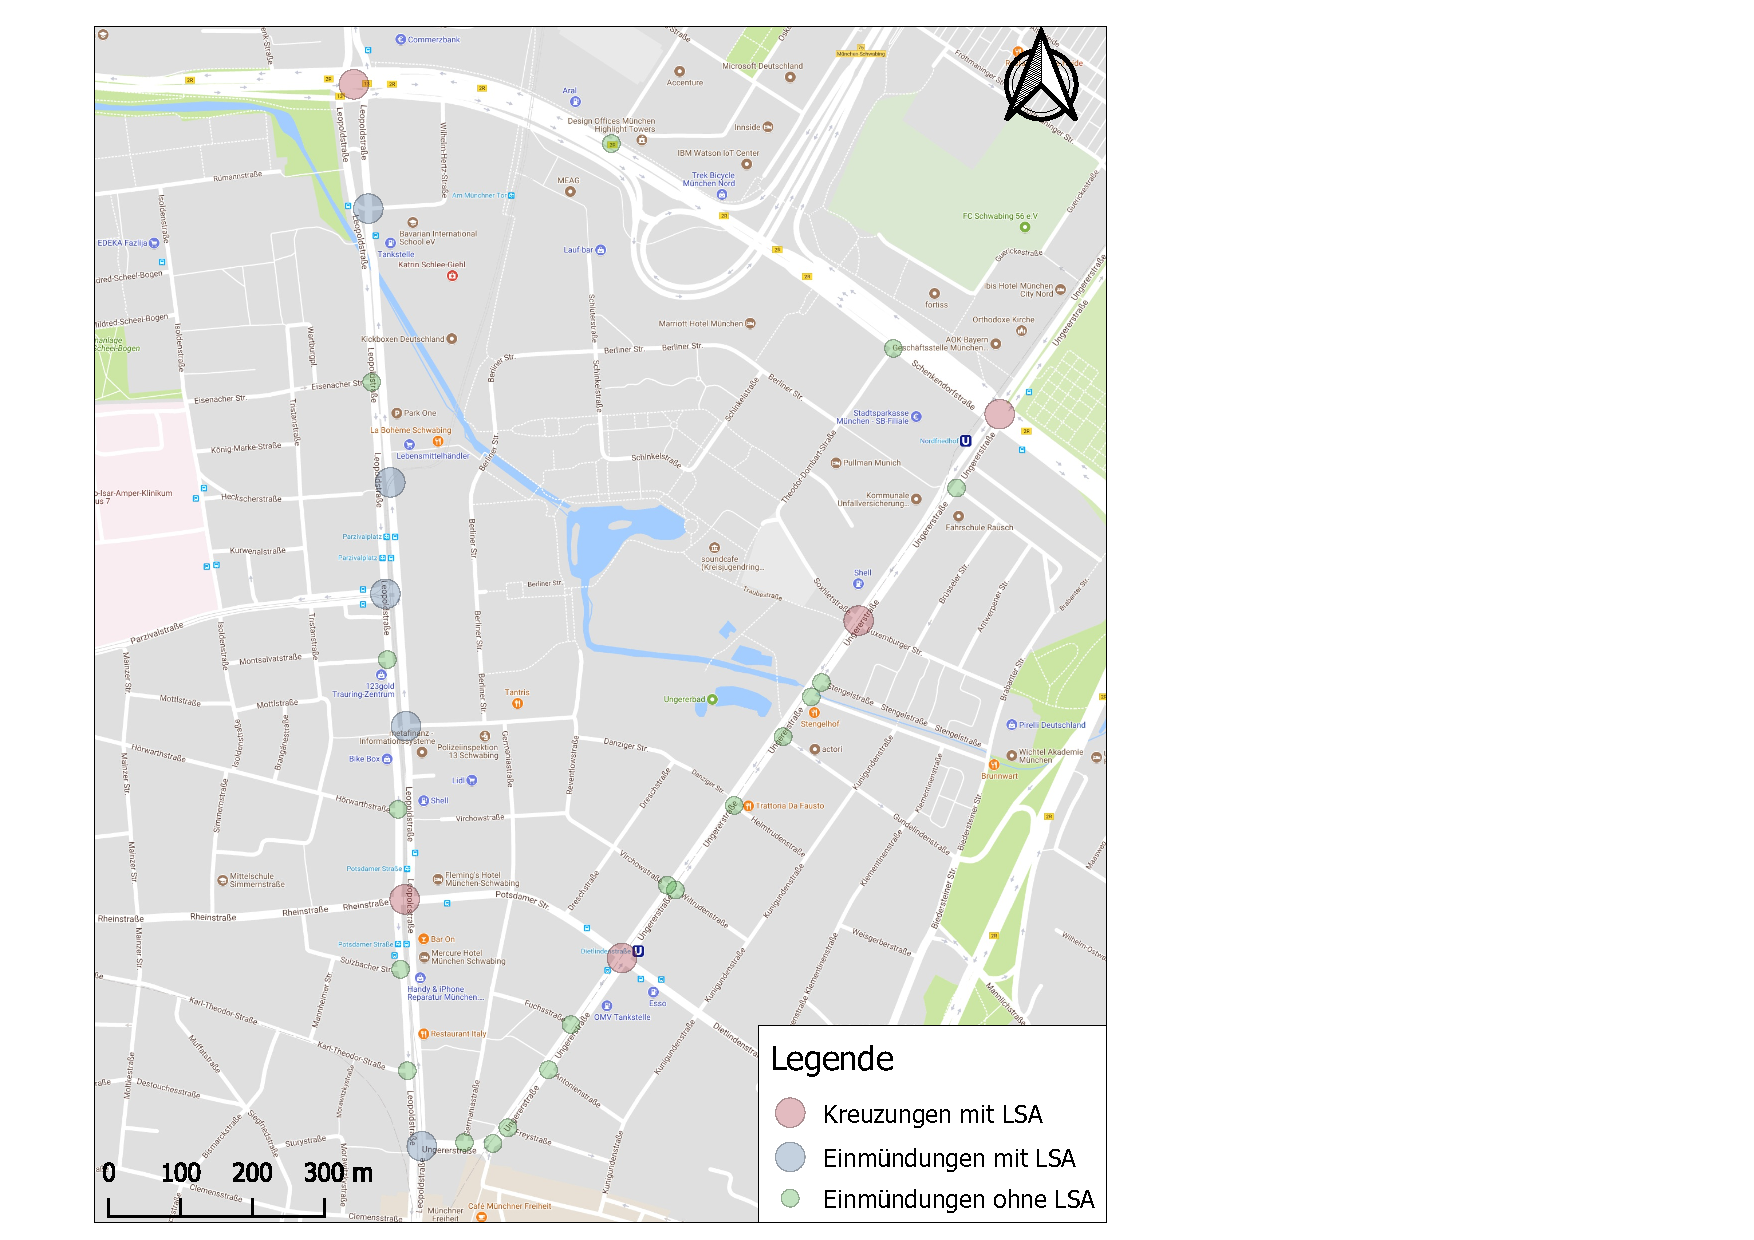
\includegraphics[width=21.5cm,height=17cm]{figures/Markante_Punkte}
		\caption[Darstellung der Teststrecke, die markierten Punkte geben Auskunft über die Art und Regelung des Knotenpunkts]{Darstellung der Teststrecke, die markierten Punkte geben Auskunft über die Art und Regelung des Knotenpunkts}\label{fig:Knoten_Testgebiet}
	\end{figure}
\end{savenotes}